\newcommand{\computationalPIR}{
    \begin{figure}
        \centering
        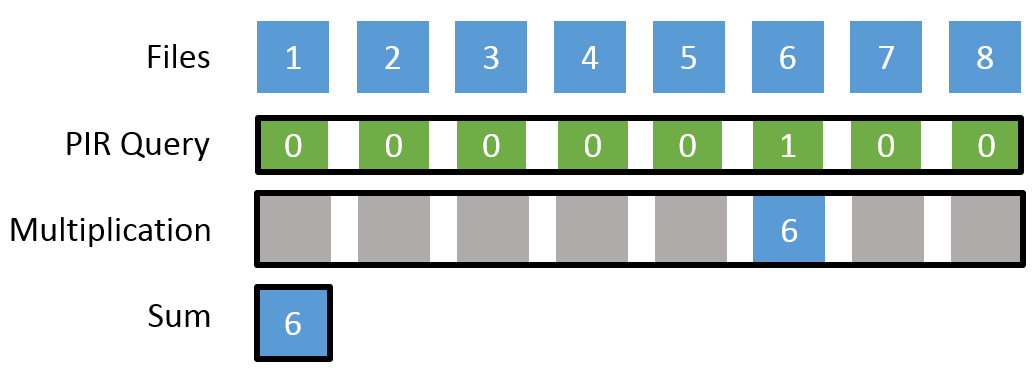
\includegraphics[width=\linewidth]{figs/pir-basic}
        \caption{Computational PIR leverages homomorphic encryption to make private queries to a database. A user encrypts a vector of 0s and a 1 corresponding to the desired entry, the server can then leverage homormorphic multiplication and homomorphic addition to return the requested entry without learning what was requested.}
        \label{fig:cpir}
    \end{figure}
}